% Author: Izaak Neutelings (April 2022)
% Inspiration:
%  https://math.stackexchange.com/questions/401745/help-understanding-complex-roots
%  https://doi.org/10.5539/jmr.v10n6p91
\documentclass[border=3pt,tikz]{standalone}
\usepackage{amsmath}
\usepackage{tikz}
\usepackage{physics}
\usepackage[outline]{contour} % glow around text
\contourlength{1.0pt}
\usetikzlibrary{3d}

\tikzset{>=latex} % for LaTeX arrow head
\usepackage{xcolor}
\colorlet{myblue}{blue!75!black}
\colorlet{mydarkblue}{blue!50!black}
\colorlet{myred}{red!65!black}
\colorlet{mydarkred}{red!40!black}
\tikzstyle{xline}=[myblue,very thick]
\tikzstyle{round xline}=[xline,line cap=round]
\tikzstyle{area}=[xline,fill=myblue!20,fill opacity=0.5]
\tikzstyle{yzp}=[canvas is zy plane at x=0]
\tikzstyle{xzp}=[canvas is xz plane at y=0]
\tikzstyle{xyp}=[canvas is xy plane at z=0]
\def\tick#1#2{\draw[thick] (#1) ++ (#2:0.11) --++ (#2-180:0.22)}
\def\N{50}


\begin{document}


% ONE REAL solutions
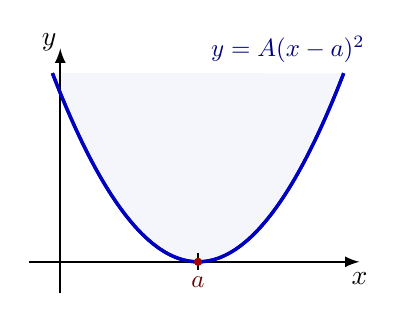
\begin{tikzpicture}[scale=1]
  \message{^^JReal solutions}
  \def\xmin{-0.4} % x axis minimum
  \def\xmax{3.8}  % x axis maximum
  \def\ymin{-0.4} % y axis minimum
  \def\ymax{2.7}  % y axis maximum
  \def\tmax{1.85} % parameter t maximum (upper)
  \def\A{0.7}     % parabola amplitude
  \def\a{1.75}    % parabola minimum
  \coordinate (M)  at (\a,0); % parabola minimum
  \coordinate (R) at (\a,0); % root
  
  % PARABOLA BACK
  \draw[area,fill opacity=0.2,samples=\N,smooth,variable=\t,domain=\a-\tmax:\a+\tmax]
    plot (\t,{\A*(\t-\a)^2});
  
  % AXES
  \draw[->,black,thick] (\xmin,0) -- (\xmax,0) node[below] {$x$};
  \draw[->,black,thick] (0,\ymin,0) -- (0,\ymax+0.01) node[anchor=-30,inner sep=1] {$y$};
  
  % PARABOLA
  \draw[xline,samples=\N,smooth,variable=\t,domain=\a-\tmax:\a+\tmax]
    plot (\t,{\A*(\t-\a)^2});
  \node[mydarkblue,left=-5,scale=0.9] at (\xmax,\ymax) {$y=A(x-a)^2$};
  
  % TICKS
  \tick{R}{90}
    node[below=-1,scale=0.9,mydarkred] {$a$};
  
  % POINTS
  \fill[myred] (M) circle(0.05);
  \fill[myred] (R) circle(0.05);
  
\end{tikzpicture}


% REAL solutions
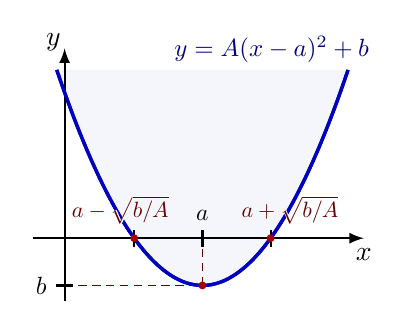
\begin{tikzpicture}[scale=1]
  \message{^^JReal solutions}
  \def\xmin{-0.4} % x axis minimum
  \def\xmax{3.8}  % x axis maximum
  \def\ymin{-0.8} % y axis minimum
  \def\ymax{2.4}  % y axis maximum
  \def\tmax{1.85} % parameter t maximum (upper)
  \def\A{0.8}     % parabola amplitude
  \def\a{1.75}    % parabola minimum
  \def\b{0.6}     % parabola vertical offset
  \pgfmathsetmacro\r{sqrt(\b/\A)} % root
  \coordinate (M)  at (\a,-\b);  % parabola minimum
  \coordinate (R+) at (\a+\r,0); % largest root
  \coordinate (R-) at (\a-\r,0); % smallest root
  
  % PARABOLA BACK
  \draw[area,fill opacity=0.2,samples=\N,smooth,variable=\t,domain=\a-\tmax:\a+\tmax]
    plot (\t,{\A*(\t-\a)^2-\b});
  
  % AXES
  \draw[->,black,thick] (\xmin,0) -- (\xmax,0) node[below] {$x$};
  \draw[->,black,thick] (0,\ymin,0) -- (0,\ymax+0.01) node[anchor=-30,inner sep=1] {$y$};
  
  % PARABOLA
  \draw[xline,samples=\N,smooth,variable=\t,domain=\a-\tmax:\a+\tmax]
    plot (\t,{\A*(\t-\a)^2-\b});
  \node[mydarkblue,left=-5,scale=0.9] at (\xmax,\ymax) {$y=A(x-a)^2+b$};
  
  % TICKS
  \draw[mydarkred,densely dashed] (0,-\b) -- (M) -- (\a,0);
  \tick{0,-\b}{0} node[left=0,scale=0.9] {$b$};
  \tick{\a,0}{-90}
    node[above=0,scale=0.85] {$a$};
  \tick{R-}{-90}
    node[left=5,above=-1,scale=0.8,mydarkred] {\contour{white}{$a-\sqrt{b/A}$}}; %\dfrac{b}{A}
  \tick{R+}{-90} 
    node[right=7,above=-1,scale=0.8,mydarkred] {\contour{white}{$a+\sqrt{b/A}$}}; %\dfrac{b}{A}
  
  % POINTS
  \fill[myred] (M) circle(0.05);
  \fill[myred] (R+) circle(0.05) (R-) circle(0.05);
  
\end{tikzpicture}


% IMAGINARY solutions
\def\ymax{2.7}  % y axis maximum
\def\tmax{1.78} % parameter t maximum (upper)
\def\tlow{1.42} % parameter t maximum (lower)
\begin{tikzpicture}[scale=1]
  \message{^^JImaginary solutions}
  \def\xmin{-2.0} % x axis minimum
  \def\xmax{2.2}  % x axis maximum
  \def\ymin{-0.8} % y axis minimum
  \def\A{0.6}     % parabola amplitude
  \def\b{0.5}     % parabola vertical offset
  \pgfmathsetmacro\r{sqrt(\b/\A)} % root
  \coordinate (M)  at (0,\b);  % parabola minimum
  \coordinate (R+) at ( \r,0); % root with positive Im[z]
  \coordinate (R-) at (-\r,0); % root with negative Im[z]
  \coordinate (P+) at ( \r,2*\b); % root with positive Im[z], shifted
  \coordinate (P-) at (-\r,2*\b); % root with negative Im[z], shifted
  
  % PARABOLA BACK
  \draw[area,fill opacity=0.2,samples=\N,smooth,variable=\t,domain=-\tmax:\tmax]
    plot (\t,{\b+\A*\t*\t});
  
  % AXES
  \draw[->,black,thick] (\xmin,0) -- (\xmax,0) node[below] {$x$};
  \draw[->,black,thick] (0,\ymin,0) -- (0,\ymax+0.01) node[anchor=-30,inner sep=1] {$y$};
  
  % PARABOLA
  \draw[xline,samples=\N,smooth,variable=\t,domain=-\tmax:\tmax]
    plot (\t,{\b+\A*\t*\t});
  \draw[area,thin,fill opacity=0.1,samples=\N,smooth,variable=\t,domain=-\tlow:\tlow]
    plot (\t,{\b-\A*\t*\t});
  \node[mydarkblue,right=4,scale=0.9] at (0,\ymax) {$y=Ax^2+b$};
  \draw[mydarkred,densely dashed] (R+) |- (0,2*\b) -| (R-);
  
  % TICKS
  \tick{0,\b}{0} node[above=1,left=-1,scale=0.9] {\contour{white}{$b$}};
  \tick{0,2*\b}{0} node[above=1,left=-1,scale=0.9] {\contour{myblue!4}{$2b$}};
  \tick{-\r,0}{90}
    node[left=2,below=-2,scale=0.9,mydarkred] {\contour{white}{$-\sqrt{b/A}$}}; %\dfrac{b}{A}
  \tick{\r,0}{90} 
    node[right=2,below=-2,scale=0.9,mydarkred] {\contour{white}{$+\sqrt{b/A}$}}; %\dfrac{b}{A}
  
  % POINTS
  \fill[myred] (M) circle(0.05);
  \fill[myred] (R+) circle(0.05) (R-) circle(0.05);
  \fill[myred] (P+) circle(0.05) (P-) circle(0.05);
  
\end{tikzpicture}


% COMPLEX solutions
\begin{tikzpicture}[scale=1]
  \message{^^JComplex solutions}
  \def\xmin{-0.6} % x axis minimum
  \def\xmax{3.5}  % x axis maximum
  \def\ymin{-0.3} % y axis minimum
  \def\A{0.6}     % parabola amplitude
  \def\a{1.4}     % parabola minimum
  \def\b{0.5}     % parabola vertical offset
  \pgfmathsetmacro\r{sqrt(\b/\A)} % root
  \coordinate (M)  at (\a,\b);   % parabola minimum
  \coordinate (R+) at (\a+\r,0); % root with positive Im[z]
  \coordinate (R-) at (\a-\r,0); % root with negative Im[z]
  \coordinate (P+) at (\a+\r,2*\b); % root with positive Im[z], shifted
  \coordinate (P-) at (\a-\r,2*\b); % root with negative Im[z], shifted
  
  % PARABOLA BACK
  \draw[area,fill opacity=0.25,samples=\N,smooth,variable=\t,domain=\a-\tmax:\a+\tmax]
    plot (\t,{\b+\A*(\t-\a)^2});
  
  % AXES
  \draw[->,black,thick] (\xmin,0) -- (\xmax,0) node[below] {$x$};
  \draw[->,black,thick] (0,\ymin,0) -- (0,\ymax+0.01) node[anchor=-30,inner sep=1] {$y$};
  
  % PARABOLA
  \draw[xline,samples=\N,smooth,variable=\t,domain=\a-\tmax:\a+\tmax]
    plot (\t,{\b+\A*(\t-\a)^2});
  \draw[area,thin,fill opacity=0.1,samples=\N,smooth,variable=\t,domain=\a-\tlow:\a+\tlow]
    plot (\t,{\b-\A*(\t-\a)^2});
  \node[mydarkblue,right=5,scale=0.9] at (0,\ymax) {$y=A(x-a)^2+b$};
  \draw[mydarkred,densely dashed] (R+) |- (0,2*\b) -| (R-);
  
  % TICKS
  \draw[mydarkred,densely dashed] (0,\b) -- (M) -- (\a,0);
  \tick{0,\b}{0} node[scale=0.9,left=-1] {$b$};
  \tick{0,2*\b}{0} node[scale=0.9,left=-1] {$2b$};
  \tick{\a,0}{90}
    node[below=1,scale=0.8] {\contour{white}{$a$}}; %\dfrac{b}{A}
  \tick{R-}{90}
    node[left=5,below=-1,scale=0.8,mydarkred] {\contour{white}{$a-\sqrt{b/A}$}}; %\dfrac{b}{A}
  \tick{R+}{90} 
    node[right=2,below=-1,scale=0.8,mydarkred] {\contour{white}{$a+\sqrt{b/A}$}}; %\dfrac{b}{A}
  
  % POINTS
  \fill[myred] (M) circle(0.05);
  \fill[myred] (R+) circle(0.05) (R-) circle(0.05);
  \fill[myred] (P+) circle(0.05) (P-) circle(0.05);
  
\end{tikzpicture}


% IMAGINARY ROOTS - extended graph
\def\xang{-10}
\def\zang{25}
\begin{tikzpicture}[y=(90:1),z=(\zang:1),x=(\xang:1),scale=1.1]
  \message{^^JImaginary solutions - extended graph}
  \def\xmax{1.8}  % x axis maximum
  \def\ymin{-1.3} % y axis minimum
  \def\ymax{2.7}  % y axis maximum
  \def\zmax{1.8}  % z axis maximum
  \def\tmax{1.0}  % parameter t maximum (upper)
  \def\tlow{1.1}  % parameter t maximum (lower)
  \def\A{1.5}     % parabola amplitude
  \def\b{0.95}    % parabola vertical offset
  \pgfmathsetmacro\r{sqrt(\b/\A)} % root
  \coordinate (M)  at (0,\b,0); % parabola minimum
  \coordinate (R+) at (0,0, \r); % root with positive Im[z]
  \coordinate (R-) at (0,0,-\r); % root with negative Im[z]
  
  % AXES
  \draw[black,thick] (-\xmax,0,0) -- (0,0,0);
  
  % PARABOLA
  \draw[area,samples=\N,smooth,variable=\t,domain=-\tlow:\tlow]
    plot (0,{\b-\A*\t*\t},\t);
  \draw[area,samples=\N,smooth,variable=\t,domain=-\tmax:\tmax]
    plot (\t,{\A*\t*\t+\b},0);
  \node[mydarkblue,right=7,scale=0.9] at (0,0.96*\ymax,0) {$y=Ax^2+b$};
  \node[mydarkblue,below=5,left=4,scale=0.9] at (0,\ymin,0) {$y=b-At^2$};
  
  % AXES
  \draw[->,black,thick] (0,\ymin,0,0) -- (0,\ymax+0.06,0) node[above left=-3] {$y$};
  \draw[->,black,thick] (0,0,-\zmax) -- (0,0,\zmax) node[right=8,above=-2] {$t=\Im[z]$};
  
  % POINTS
  \tick{0,\b,0}{0} node[left=1] {$b$};
  \fill[myred] (M) circle(0.05);
  \fill[myred,xzp]
    (R+) circle(0.05)
    (R-) circle(0.05);
  
  % FRONT
  \draw[round xline,samples=\N,smooth,variable=\t]
    plot[domain=0.006-\r:-0.01] (0,{\b-\A*\t*\t},\t)
    plot[domain=\r/2:\r-0.008] (0,{\b-\A*\t*\t},\t);
  \draw[->,black,thick,line cap=round]
    (0.01,0,0) -- (\xmax,0,0) node[right=5,below=0] {$x=\Re[z]$};
  
  % TICKS
  \tick{R-}{-90} node[mydarkred,scale=0.9,anchor=-5,inner sep=2] {$-\sqrt{b/A}$};
  \tick{R+}{90} node[mydarkred,scale=0.9,anchor=186,inner sep=2] {$+\sqrt{b/A}$};
  
\end{tikzpicture}


% COMPLEX ROOTS - extended graph
\def\xang{-7}
\def\zang{25}
\begin{tikzpicture}[y=(90:1),z=(\zang:1),x=(\xang:1),scale=1.2]
  \message{^^JComplex solutions - extended graph}
  \def\xmax{3.2}  % x axis maximum
  \def\ymin{-1.3} % y axis minimum
  \def\ymax{2.8}  % y axis maximum
  \def\zmin{-1.6} % z axis minimum
  \def\zmax{2.4}  % z axis maximum
  \def\tmax{1.00} % parameter t maximum (upper)
  \def\tlow{1.10} % parameter t maximum (lower)
  \def\A{1.5}     % parabola amplitude
  \def\a{1.5}     % parabola minimum
  \def\b{1.1}     % parabola vertical offset
  \pgfmathsetmacro\r{sqrt(\b/\A)} % root
  \coordinate (M)  at (\a,\b,0); % parabola minimum
  \coordinate (R+) at (\a,0, \r); % root with positive Im[z]
  \coordinate (R-) at (\a,0,-\r); % root with negative Im[z]
  
  % AXES
  \draw[black,thick] (-0.1*\ymax,0,0) -- (\a,0,0);
  \draw[->,black,thick] (0,\ymin,0,0) -- (0,\ymax,0) node[above left=-3] {$y$};
  \draw[->,black,thick] (0,0,\zmin) -- (0,0,\zmax) node[above=1,right=1] {$t=\Im[z]$};
  \draw[mydarkred,densely dashed]
    (R+) -- (0,0,\r);
  
  % PARABOLA
  \draw[area,samples=\N,smooth,variable=\t,domain=-\tlow:\tlow]
    plot (\a,{\b-\A*\t*\t},\t);
  \draw[area,samples=\N,smooth,variable=\t,domain=\a-\tmax:\a+\tmax]
    plot (\t,{\b+\A*(\t-\a)^2},0);
  \node[mydarkblue,right=2,scale=0.9] at (\a,\ymax,0) {$y=A(x-a)^2+b$};
  \node[mydarkblue,right=0,scale=0.9] at (0.6*\a,0.9*\ymin,0) {$y=b-At^2$ ($x=a$)};
  
  % POINTS
  \fill[myred] (M) circle(0.05);
  \fill[myred,xzp]
    (R+) circle(0.05)
    (R-) circle(0.05);
  \draw[mydarkred,densely dashed]
    (M) -- (0,\b,0)
    (R-) -- (0,0,-\r)
    (R+) -- (R-);
  
  % FRONT
  \draw[round xline,samples=\N,smooth,variable=\t]
    plot[domain=0.006-\r:-0.01] (\a,{\b-\A*\t*\t},\t)
    plot[domain=\r/2:\r-0.008] (\a,{\b-\A*\t*\t},\t);
  \draw[->,black,thick,line cap=round]
    (\a,0,0) -- (\xmax,0,0) node[right=5,below=0] {$x=\Re[z]$};
  
  % TICKS
  \tick{\a,0,0}{90} node[below=-1] {$a$};
  \tick{0,0,-\r}{-90}
    node[mydarkred,scale=0.9,anchor=-40,inner sep=0] {$-\sqrt{b/A}$};
  \tick{0,0,\r}{-90}
    node[mydarkred,scale=0.9,anchor=-40,inner sep=0] {$+\sqrt{b/A}$};
  \tick{0,\b,0}{0} node[left=0] {$b$};
  
\end{tikzpicture}


% QUADRATIC EQUATION
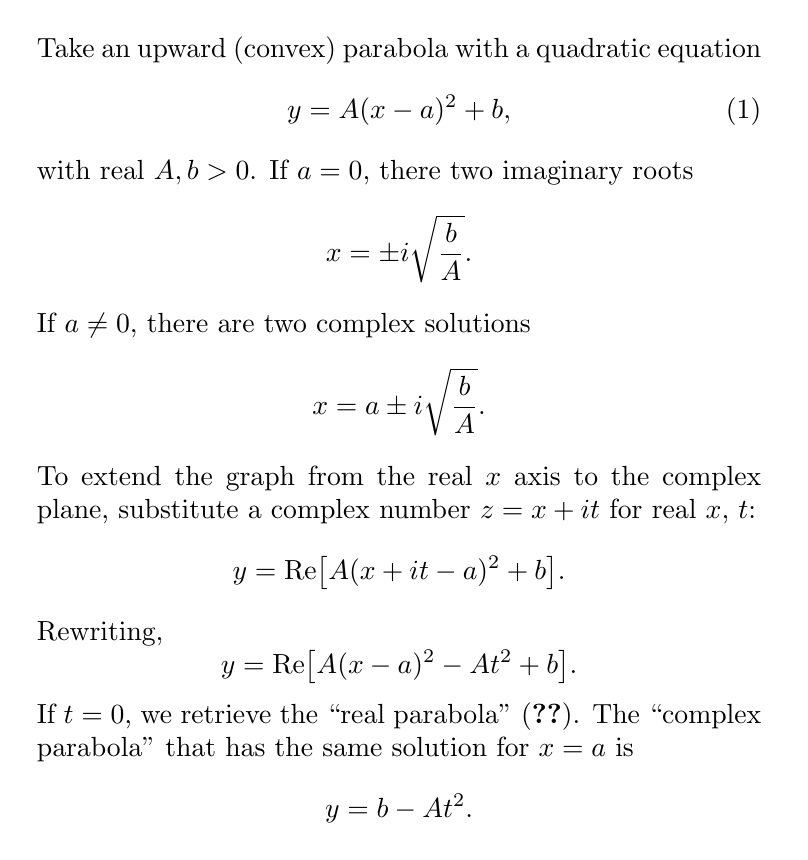
\begin{tikzpicture}[scale=1]
  \node[align=left] at (0,0) {
    \begin{minipage}{9.2cm}
      Take an upward (convex) parabola with a quadratic equation
      \begin{equation}\label{real}
        y = A(x-a)^2 + b,
      \end{equation}
      with real $A,b>0$.
      If $a=0$, there two imaginary roots
      \begin{equation*}
        x = \pm i\sqrt{\frac{b}{A}}.
      \end{equation*}
      If $a\neq0$, there are two complex solutions
      \begin{equation*}
        x = a \pm i\sqrt{\frac{b}{A}}.
      \end{equation*}
      To extend the graph from the real $x$ axis to the complex plane,
      substitute a complex number \mbox{$z = x + it$} for real $x$, $t$:
      \begin{equation*}
        y = \Re\!\big[ A(x+it-a)^2 + b \big].
      \end{equation*}
      Rewriting,
      \begin{equation*}
        y = \Re\!\big[ A(x-a)^2 -At^2 + b \big].
      \end{equation*}
      If $t=0$, we retrieve the ``real parabola'' \eqref{real}.
      The ``complex parabola'' that has the same solution for $x=a$ is
      \begin{equation*}
        y = b -At^2.
      \end{equation*}
    \end{minipage}
  };
\end{tikzpicture}


\end{document}